\documentclass[17pt]{beamer} %Makes presentation
%\documentclass[handout]{beamer} %Makes Handouts
\usetheme{Singapore} %Gray with fade at top
\useoutertheme[subsection=false]{miniframes} %Supppress subsection in header
\useinnertheme{rectangles} %Itemize/Enumerate boxes
\usecolortheme{seagull} %Color theme
\usecolortheme{rose} %Inner color theme

\definecolor{light-gray}{gray}{0.75}
\definecolor{dark-gray}{gray}{0.55}
\setbeamercolor{item}{fg=light-gray}
\setbeamercolor{enumerate item}{fg=dark-gray}

\setbeamertemplate{navigation symbols}{}
%\setbeamertemplate{mini frames}[default]
%\setbeamercovered{dynamics}
\setbeamerfont*{title}{size=\Large,series=\bfseries}
\setbeamerfont{footnote}{size=\tiny}

%\setbeameroption{notes on second screen} %Dual-Screen Notes
%\setbeameroption{show only notes} %Notes Output

\setbeamertemplate{frametitle}{\vspace{.5em}\bfseries\insertframetitle}
\newcommand{\heading}[1]{\noindent \textbf{#1}\\ \vspace{1em}}

\usepackage{bbding,color,multirow,times,ccaption,tabularx,graphicx,verbatim,booktabs}
\usepackage{colortbl} %Table overlays
\usepackage[english]{babel}
%\usepackage[latin1]{inputenc}
%\usepackage[T1]{fontenc}
\usepackage{lmodern}

%\author[]{Thomas J. Leeper}
\institute[]{
  \inst{}%
  Department of Government\\London School of Economics and Political Science
}

\usepackage{tikz}
\usetikzlibrary{shapes,arrows,positioning}

\title{Building and Testing Political Science Theories}

% How do we create social science theories based on past evidence and novel observation? What roles do induction and deduction play in contemporary political science?

\date[]{}

\begin{document}

\frame{\titlepage}

\frame{\tableofcontents}

\section{Finish Measurement}
\frame{\tableofcontents[currentsection]}


\frame{

\frametitle{{\large Assessing Measurement Quality}}

\begin{enumerate}\itemsep1em
\item Conceptual clarity
\item Construct validity
	\begin{itemize}
	\item Convergent validity
	\item Divergent validity
	\end{itemize}
\item Accuracy and precision
\end{enumerate}

}

\frame{
\frametitle{Assessing Measures I}

\begin{itemize}\itemsep1em
\item Conceptual clarity is about knowing what we want to measure
\item Sloppy concepts make for bad measures
	\begin{itemize}
	\item Ambiguity % multiple meanings or multiple labels
	\item Vagueness % concept without a definition
	\end{itemize}
\item<2-> Revise concept definition as needed
\end{itemize}
}


\frame{
\frametitle{Assessing Measures II}

\begin{itemize}\itemsep0.5em
\item Construct validity is the degree to which a variable measures a concept\footnote{Note: Kellstedt and Whitten call this ``content validity''. They use ``construct validity'' to mean whether a measure has predictive validity (i.e., that the measure is related to measures of other concepts that are theorized to be related).}
\item<2-> Construct validity is \textbf{high} if a variable is a measure of the concept we care about
\item<3-> Construct validity is \textbf{low} if a variable is actually a measure of something else
\end{itemize}
}

% sources: bad concept definition; totally inappropriate measures (using income to measure weight); measure becomes the concept (actual income is replaced by self-reported income)

\frame{

\frametitle{{\large Assessing Construct Validity}}

\begin{itemize}\itemsep1em
\item Multiple measures!
\item Convergence (Convergent validity)
\item Discrimination (Discriminant validity)
\end{itemize}
}

% two (or more) measures of the same concept are highly correlated; scaling
% two (or more) measures of distinct concepts are not correlated
% Measures of distinct concepts may be correlated if they are causally related to one another, so simple correlations do not mean two measures are necessarily of the same concept

% mention predictive validity (what Kellstedt and Whitten call construct validity)


\frame{}


\section{Theory}
\frame{\tableofcontents[currentsection]}



\frame{
\frametitle{Scientific method}

\begin{enumerate}
\item Research question(s)
\item Clarify the core concepts
\item \textbf{Develop theory}
\item Derive specific, testable hypotheses
\item Plan data collection
\item Gather data/evidence
\item Analyze data
\item Draw inferences
\end{enumerate}

}

\frame{
\frametitle{{\large Key Points from Last Week}}

\begin{enumerate}\itemsep1em
\item Theory is about concepts
\item Analysis is about measured variables
\item So our task as scientists is to:
	\begin{itemize}
	\item Find observable implications of theory
	\item Draw theoretical implications from measures
	\end{itemize}
\end{enumerate}
}


\frame{

\begin{center}
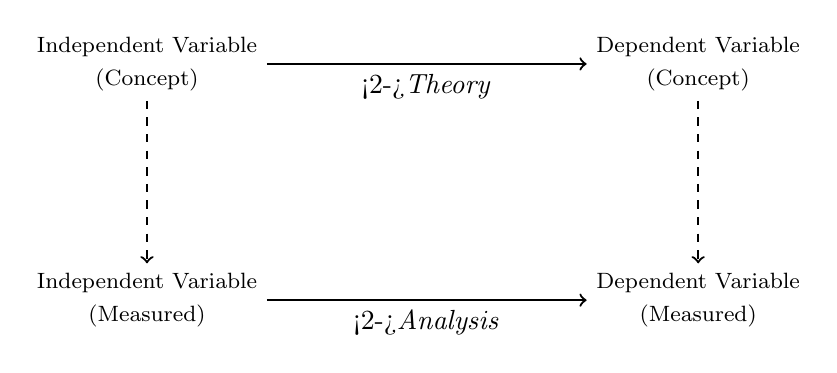
\begin{tikzpicture}
\node [align=center] (ivm) at (0,0) {\footnotesize Independent Variable\\\footnotesize (Measured)};
\node [align=center] (dvm) at (7,0) {\footnotesize Dependent Variable\\\footnotesize (Measured)};

\node [align=center] (ivc) at (0,3) {\footnotesize Independent Variable\\\footnotesize (Concept)};
\node [align=center] (dvc) at (7,3) {\footnotesize Dependent Variable\\\footnotesize (Concept)};

\node (analysis) at (3.5, 0) {};
\node (theory) at (3.5, 3) {};

\draw [->, thick] (ivm) -- (dvm) node[midway, below] (analysis) {{\only<2->{\textit{Analysis}}}};
\draw [->, thick] (ivc) -- (dvc) node[midway, below] (theory) {{\only<2->{\textit{Theory}}}};
\draw [->, dashed, thick] (ivc) -- (ivm);
\draw [->, dashed, thick] (dvc) -- (dvm);
\end{tikzpicture}
\end{center}


}


\frame{}

\frame{

\frametitle{{\large What is a theory?}}

\begin{itemize}\itemsep1em
\item Kellstedt and Whitten's definition:\footnote{Kellstedt and Whitten, p.3}\\
A tentative conjecture about the causes of some phenomenon of interest
\item<2-> Another way of saying this:\\
An \alert<3>{argument} that attempts to \alert<3>{explain} how concepts are causally related
\end{itemize}

}

% theories are arguments and they are (potential) explanations
% concepts may also be hierarchical - some are grand, macro theories; others are small micro theories and it may be that the micro theories build on macro theories

% there are also descriptive theories, e.g., typologies (Presidential character, welfare states, )



\frame{

\frametitle{Generating Theory I}

\begin{itemize}\itemsep0.5em
\item One way to theorize is to reason \textit{inductively} % bottom-up appraoch

\item Induction works by drawing generalities from specific observations

\item Sometimes called ``bottom-up'' theorizing
\end{itemize}

}

% activity to practice inductive reasoning
%% why do people vote or why do people not vote?

%% perhaps gender differences in female legislative representation?


\frame{

\frametitle{Generating Theory II}

\begin{itemize}\itemsep0.5em
\item An alternative way of developing theory is through \textit{deduction} 

\item Deduction begins from general, assumed principles/axioms to reach more specific observable realities % top-down approach

\item<2-> Common example: Rational choice theory

\end{itemize}

}

% the first calculus of voting (Arrow; Downs) was purely deductive


\frame<1>[label=theory1]{

\frametitle{Generating Theory III}

\begin{itemize}\itemsep0.5em
\item ``The Calculus of Voting'' is a \textit{rational choice} theory
	\begin{itemize}
	\item Assumes utility maximization is the driver of all behaviour
	\item Understanding phenomena is a matter of figuring out utility structures, especially those created by institutions
	\end{itemize}
\item<2-> Not the only broad theoretical paradigm
\end{itemize}
}


\frame{

\frametitle{The Calculus of Voting}

\small

Theory: Voting is explained by \only<1>{3}\only<2>{4} factors\\

\begin{columns}
  \begin{column}{0.45\textwidth}
    \begin{itemize}
	\item Costs of voting
	\item Benefits from preferred alternative winning
	\item Probability of impacting result
	\item<2-> Benefits from voting \textit{per se}
    \end{itemize}
  \end{column}
  
  \begin{column}{0.55\textwidth}
  \tikzstyle{block} = [rectangle, draw, text width=2cm, text centered, rounded corners, minimum height=1em, node distance=9cm]
  \begin{tikzpicture}[scale=0.3]
  \draw<1-> [block] node at (0,0) (voting) {{\small Pr(Voting)}};
  \draw<1-> [block, above left of=voting] node (costs) {{\small Costs}};
  \draw<1-> [block, left of=voting] node (ben) {{\small Benefits}};
  \draw<1-> [block, below left of=voting] node (p) {{\small Pr(Impact)}};
  \draw<2-> [block, below of=voting] node (d) {{\small ``D term''}};
  \draw<1-> [->, very thick] (costs) -- (voting);
  \draw<1-> [->, very thick] (ben) -- (voting);
  \draw<1-> [->, very thick] (p) -- (voting);
  \draw<2-> [->, very thick] (d) -- (voting);
  \end{tikzpicture}
  
  \end{column}
\end{columns}

}


% other examples of this:
% logic of collecive action; selective incentives; Mancur Olson
% common pool resource problems; communication and sanctions; Elinor Ostrom

% an example: calculus of voting



\frame{

\frametitle{Aside: Assumptions}

\begin{center}
If a theory require assumptions, is that theory credible?
\end{center}

}

% there are debates about whether it is okay to make assumptions that we do not test (see, e.g., Kahneman and Tversky)
% there are also debates about whether theories are useful independent of whether they explain the world as it is (see, e.g., Clark and Primo)

\againframe{theory1}



\frame{

\frametitle{The Michigan Model}

\small

Theory: Vote choice is explained by long-standing partisan identification, which is in turn shaped by early socialization.

\vspace{2em}

\tikzstyle{block} = [draw, text width=2.5cm, minimum height=1em, node distance=8cm]
\begin{tikzpicture}[scale=0.75]
\draw [block] node at (0,0) (voting) {{\small Vote Choice}};
\draw [block] node at (-5,0) (pid) {{\small Party\\ Identification}};
\draw [block] node at (-10,1.5) (p) {{\small Parental\\ Party ID}};
\draw [block] node at (-10,-1.5) (e) {{\small Early Adult\\ Experiences}};
\draw [->, very thick] (p) -- (pid);
\draw [->, very thick] (e) -- (pid);
\draw [->, very thick] (pid) -- (voting);
\end{tikzpicture}
}




\frame{

\frametitle{Induction vs. Deduction?}

\begin{itemize}\itemsep0.5em
\item Induction and deduction are both integral to science

% example: the calculus of voting; modified theory based on new evidence

\item Theory testing and theory building both require observation
\end{itemize}

}

% the second calculus of voting (Riker and Ordeshook) was partly inductive

% theory development is separate from theory testing
% but the two are interrelated



% induction (bottom up) vs. deduction (top down; from theory to observation)
% generally, in political science, we are interested in building theories from earlier more acceptable theoretical premises
% if we believe the world operates in some way, we can draw more specific conjectures about features of the world
% and then test those conjectures using evidence

% yet, the result is that when we collect evidence, sometimes we falsify (or fail to find evidence in support of) our theories
% the results is that we must either amend our premises, amend our argument, or set scope conditions on theory

% these theories then become useful because by drawing generalities about the world, we are able to understand particular events
% when those particular events then deviate from expectations, it invites renewed theorizing, amendment of argument, or the implication of scope conditions

% so science is both deductive and inductive, though the way we talk about science is typically deductive


% in the end, however, our goal is to "explain" the world...that has to start from a mix of assumption-based theory, theory development expanding on previously validated theory, and novel data collection


\frame{

\frametitle{Theory Generation in Practice}

As you theorize an explanation for some phenomenon, you will draw on:

\begin{itemize}\itemsep1em
\item General principles
\item Extant theory
% application; generalization; moderation; scope conditions; proposing mechanisms for extant relationships
\item Specific evidence
% don't use the evidence we will eventually test our theory on
\end{itemize}

}


\frame{

\frametitle{{\large What makes for a good theory?}}

\begin{itemize}
\item Truth
\item Falsifiability
\item Relevance
\item Coherence
\item Generality
\item Parsimony
\end{itemize}

}

\frame{

\frametitle{Generality \& Parsimony}

Think for 90 seconds about each of these principles:

\small 

\begin{itemize}\itemsep1em
\item Generality: Theories that can explain more are preferred over theories that can explain less
\item Parsimony: Simple theories are preferred over complex theories
\end{itemize}

\normalsize

Are these principles defensible?\\ Are they any good?

}



\frame{}


\section{Preview Next Week}
\frame{\tableofcontents[currentsection]}

\frame{
\frametitle{Preview}

\begin{itemize}\itemsep0.5em
\item Drawing inferences requires tests
\item Testing theories requires observation of reality
\item Focus on two tasks:
	\begin{itemize}
	\item Generating specific ``observable implications'' of theories
	\item Discuss how to distinguish between rival theories
	\end{itemize}
\end{itemize}
}

% evidence + rules for evaluating evidence
%% what counts as evidence and rules for evaluating evidence vary quite a bit

% broadly, we "test" theories by drawing observable implications of those theories, such that the theories are "observationally inequivalent" (each theory would produce different expectations about how the world would look), and then updating our beliefs about the alternative theories (such that the one more consistent with evidence is more likely to be "true")

% there is no truth, there are only beliefs about the true nature of the world


\appendix
\frame{}

\end{document}
